\chapter{Personendetektion}
\label{chap:Personendetektion}


Dieser Abschnitt beschreibt das Vorgehen, um die Anzahl Personen in einem Aufzug zu erkennen. In einem ersten Schritt wird die Verarbeitung der Rohdaten aufgezeigt. Für den Auswertealgorithmus wurden mehrere unterschiedliche Aufzüge evaluiert und ein Profil erstellt. 



\begin{figure}[H]
	\centering
	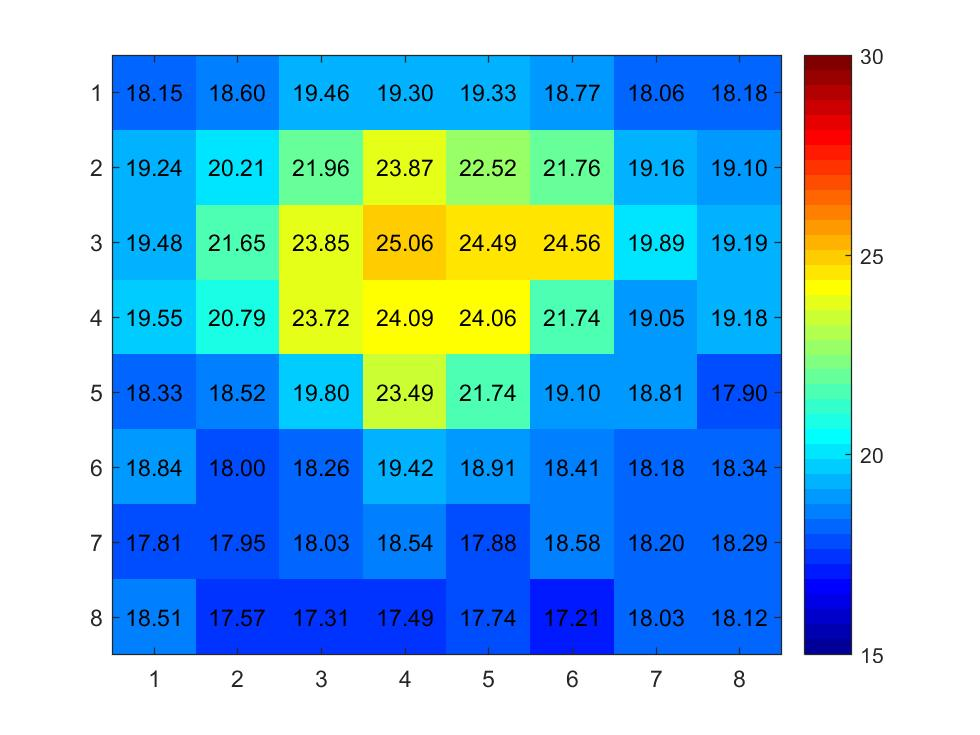
\includegraphics[width=0.5\textwidth]
	{fig/person_175_shirt.jpg}
	\caption[Pixeldarstellung einer Person]{Pixeldarstellung einer Person}
	\label{fig:Pixelbild}
\end{figure}



\section{Datenverarbeitung}




\section{Datenmanipulation mittels Interpolation}

Die Auflösung von 8x8 Pixel bietet optisch nur begrenzte Aussagekraft über die Anzahl Personen in einem Aufzug. Daher wurde mittels MATLAB mehrere Interpolationsverfahren benutzt, um die Auflösung der Personenerkennung zu verbessern. Im Zusammenhang mit den Pixelwerten eignet sich eine bikubische



Da im Zusammenhang mit dem Auswertealgorithmus mittels TensorFlow


\section{Aufbau neuronales Netzwerk}


Convolutional Networks work by moving small filters across the input image. This means the filters are re-used for recognizing patterns throughout the entire input image. This makes the Convolutional Networks much more powerful than Fully-Connected networks with the same number of variables. This in turn makes the Convolutional Networks faster to train




The convolutional filters are initially chosen at random, so the classification is done randomly. The error between the predicted and true class of the input image is measured as the so-called cross-entropy. The optimizer then automatically propagates this error back through the Convolutional Network using the chain-rule of differentiation and updates the filter-weights so as to improve the classification error. This is done iteratively thousands of times until the classification error is sufficiently low.


(W -F +2P) : S+ 1

\section{Convolution Neural Network}


\begin{figure}[H]
	\centering
	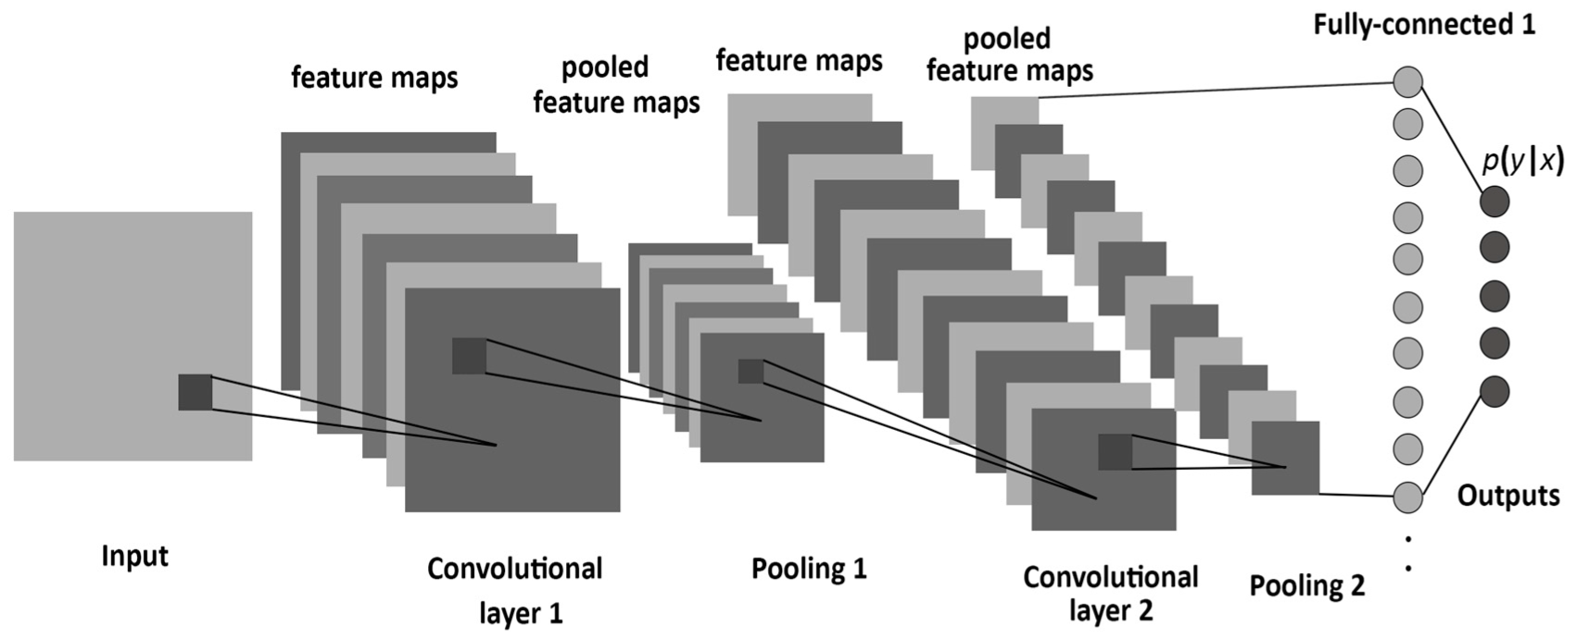
\includegraphics[width=1\textwidth]
	{fig/CCN.png}
	\caption[Aufbau des Convolutional Neural Network]{Aufbau des Convolutional Neural Network}
	\label{fig:CCN}
\end{figure}



\subsection{Profilbildung}




Profil 1
Size of:
- Training-set:         126936
- Validation-set:       25000

Profil 2



Profil 3


Testprofil Test-set:             22169

\section{Symmetrische Erweiterung}

Um die Datensätze zu vergrößern wurden die drei Profile erweitert. 



\section{Musterauswertung}







\section{c}

Entweder alle Sekunde der Mittelwert auswerten, doer alle 100 ms die Daten auswerten 

\section{Ergebnisse}

\section{Echtzeitpersonenerkennung}

Dank der Saver-Klasse von Tensorflow lassen sich erstellte CNN-Modell als ckpt-File speichern. Dabei werden alle trainierten Bias und Gewichtungen in ein ckpt-File gespeichert. Diese lassen sich wiederum in ein untrainiertes CNN laden.

Auf dieser Grundlage wurde eine Messeinheit erstellt, welche mittels trainiertenn CNN zur Echtzeit Personerkennungen durchführt. Die Messeinheit besteht aus einenm AMG8834 Eval Kit, einem Raspbery Pi3 und einer Powerbank.



 

\section{Fazit}




